\chapter{GIỚI THIỆU} \label{sec:chapter_1}
\section{Đặt vấn đề}
Sự giới hạn của phổ tần số là hạn chế của cho việc tăng độ phổ biến và dung lượng kênh truyền. Theo CISCO \cite{cisco}, số lượng thiết bị kết nối vào mạng IP sẽ nhiều hơn gấp 3 lần dân số thế giới vào năm 2023. Cụ thể, sẽ có trung bình 3.6 thiết bị trên một người năm 2023, so với 2.4 thiết bị trên một người 2018. Kết nối \ac{m2m} sẽ chiếm một nửa các kết nối trên toàn cầu vào năm 2023 (tăng từ 33 \% năm 2018 lên 50 \% vào năm 2023), và sẽ có 14.7 tỷ kết nối \ac{m2m} vào năm 2023. Hơn 70 \% dân số thế giới có thiết bị kết nối di động năm 2023. Lưu lượng di động trung bình của một người trên một tháng tăng gấp 6 lần từ năm 2017 đến năm 2022.
Sự tăng số lượng các thiết bị và nhu cầu sử dụng là nguyên nhân chính cho việc tăng lưu lượng dữ lượng di động. 
\begin{figure} [ht]
\centering
\captionsetup{justification=centering}
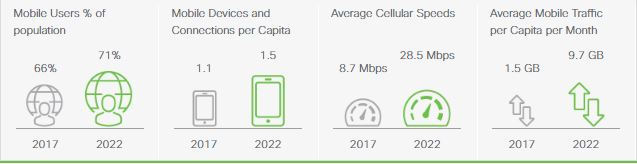
\includegraphics [scale=0.9] {Image/cisco_forecast}
\caption{Dự đoán của Cisco về dữ liệu di động \cite{cisco_forecast}}
\end{figure}
Mặc dù các nhà cung cấp dịch vụ không dây đang triển khai thêm cơ sở hạ tầng bằng cách bổ sung những trạm phát Wi-fi, nhưng hạn chế là việc sử dụng quá mức phổ \ac{rf} hiện có. Từ đó gây ra can nhiễu và chồng lấn phổ làm tăng độ trễ và giảm dung lượng. Để khắc phục tình trạng trên, một công nghệ mới đã và đang được phát triển đó là \ac{vlc} ứng dụng trong \ac{ssl} hoặc công nghệ hiển thị độ phân giải cao. Mặc dù hệ thống \ac{vlc} dùng \ac{led} chiếm tỷ lệ vượt trội khi hỗ trợ tốc độ dữ liệu cao, giá rẻ, ... Tuy nhiên với sự phát triển vượt bậc trong nhưng năm gần đây, cùng với những ưu điểm như như màu sắc dễ chịu, khả năng kiểm soát màu sắc tốt, diện tích phát xạ lớn, ...\ac{oled} được kỳ vọng sẽ trở thành công nghệ phát sáng quan trọng trong tương lai.

Hiện nay, trong các hệ thống thông tin quang \ac{vlc} đa phần dùng kiểu điều chế \ac{ofdm}.  Việc điều chế bằng \ac{ofdm} có ưu điểm là giúp cho băng thông của tín hiệu tiết kiệm được rất nhiều. Nếu dùng \ac{led} đơn có thể đạt đến 3Gbps cho khoảng băng thông khoảng 380Mhz tương ứng với 7.89bits/s/Hz trong khoảng cách 5cm, và khoảng 80Mbits/s trong 20Mhz tương ứng 4bits/s/Hz trong khoảng cách 1m. Nhưng có một khuyết điểm là \ac{ofdm} xử lý tín hiệu phức tạp trong miền \ac{dsp}, vì ngoài việc xử lý qua nhiều giai đoạn, \ac{ofdm} rất dễ nhạy cảm với việc trôi tần số nên ta cần các thuật toán và phần cứng để đồng bộ bước sóng quang và tần số phần điện. Vì vậy, ngoài việc tiếp cận bằng \ac{ofdm} thì có nhiều cách tiếp cận khác để nâng hiệu quả sử dụng băng thông, trong đó có phương pháp điều chế \ac{ook} sử dụng mã đường truyền \ac{nrz}.

Do đó, đề tài nghiên cứu việc ứng dụng neural network vào giải điều chế tín hiệu \ac{nrz} trong hệ thống \ac{vlc} dùng \ac{oled}. 

Câu hỏi nghiên cứu đặt ra của luận văn là: 
\begin{itemize}
\item Phương pháp neural network có tốt hơn phương pháp giải điều chế truyền thống hay không?
\item Mô hình và thông số nào của neural network phù hợp nhất cho việc giải điều chế?
\item Mô hình và phương pháp nào là cách tốt nhất cho việc tiền xử lý dữ liệu.
\end{itemize} 

Trong chương \ref{sec:chapter_2}, cơ sở lý thuyết về hệ thống \ac{vlc}, neural network và các phương pháp tiền xử lý sẽ được trình bày. Trong chương \ref{sec:chapter_3}, các kết quả đo đạc và giải điều chế sẽ được so sánh và phân tích. Cuối cùng, chương \ref{sec:chapter_4} đưa ra kết luận chung.

\section{Phạm vi và phương pháp nghiên cứu}
\begin{itemize}
\item Phạm vi: thử nghiệm việc giải điều chế \ac{nrz} dùng 3 phương pháp neural networks.
\item Phương pháp nghiên cứu: đo đạc tại lab 209B1, với hệ thống quang không dây dùng \ac{oled}. Các phương pháp để tiền xử lý dữ liệu gồm có \ac{cwt}, framing, \ac{dae}. Các phương pháp sử dụng để giải điều chế là \ac{pnn}, \ac{grnn}, \ac{dtnn}.
\end{itemize}
\section{Các đóng góp}
\begin{itemize}
\item Đo đạc tín hiệu \ac{nrz} và xung lorentz trên hệ thống \ac{vlc} dùng \ac{oled}, tính toán \ac{snr}, \ac{ber} và xử lý dữ liệu thu được từ osciloscope để đưa vào mô hình phân loại.
\item Xây dựng thành công các mô hình neural network cho phép phân loại các mức tín hiệu \ac{nrz} và xung lorentz và so sánh của những mô hình trên.
\item Nghiên cứu những phương pháp tiền xử lý để gia tăng độ chính xác cho mô hình phân loại.
\end{itemize}